\documentclass[tikz, border=2pt]{standalone}
\usepackage{tikz}
\begin{document}
    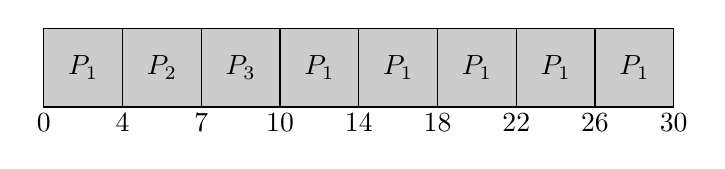
\begin{tikzpicture}
        \foreach \x in {0,...,7}
            \draw[fill=black!20] (\x,0) rectangle (\x+1,1);
        \node at (0.5,0.5) {$P_1$};
        \node at (1.5,0.5) {$P_2$};
        \node at (2.5,0.5) {$P_3$};
        \node at (3.5,0.5) {$P_1$};
        \node at (4.5,0.5) {$P_1$};
        \node at (5.5,0.5) {$P_1$};
        \node at (6.5,0.5) {$P_1$};
        \node at (7.5,0.5) {$P_1$};
        \node at (0,-0.2) {0};
        \node at (1,-0.2) {4};
        \node at (2,-0.2) {7};
        \node at (3,-0.2) {10};
        \node at (4,-0.2) {14};
        \node at (5,-0.2) {18};
        \node at (6,-0.2) {22};
        \node at (7,-0.2) {26};
        \node at (8,-0.2) {30};
    \end{tikzpicture}
\end{document}